\lstset{style=plain}

\chapter{Evaluation} \label{evaluation}

The main goal of this chapter is to give some insights about the factors that affect performance and compare different variants of the synthesis procedure described in Chapter~\ref{ch:definitions}. The chapter also puts our synthesis procedure in relation with the related work discussed in Chapter~\ref{ch:relatedwork}.


\section{Experimental set up}
This section presents the set up of the two experiments we are going to discuss in the rest of the chapter.

The goal of the first experiment is to assess the quality and the performance of the synthesiser on standard benchmarks. The detailed set up is described in Section~\ref{Evaluation on benchmarks} and the results are discussed in Section~\ref{Factors affecting runtime}.

In the second experiment the synthesiser is used to automatically generate a \emph{black list} that can be successively be used to prune the search space. We refer back to Section~\ref{Black list} for a description of pruning based on black lists. Section~\ref{Black list generation} describes how we used the synthesis procedure to generate a black list and Section~\ref{Automatic black list} reviews the quality of the generated black list.

\subsection{Evaluation on benchmarks}\label{Evaluation on benchmarks}
We evaluated $9$ variants of our synthesis procedure, crossing the $3$ exploration strategies with $3$ of the cost functions described in Chapter~\ref{ch:definitions}. The three exploration strategies we evaluated are the following.
\begin{description}
\item[plain] implements the basic synthesis procedure based on best first search described in Section~\ref{Exploration}.
\item[blacklist] implements the pruning of the search space based on a manually compiled black list provided in Table~\ref{fig:manual_black_list}. We refer to Section~\ref{Black list} for more details.
\item[template] implements the double best first search introduced in Section~\ref{Templates}. As you probably recall, the procedure first looks for a \emph{template} featuring at most \lstinline?nof_comp? higher-order components and at most \lstinline?nof_hol? holes and as soon as such a template is found the procedure falls back on the \lstinline?plain? variant up to a certain depth using only the first-order components.
\end{description}
For each exploration strategy, we instantiated the cost function with $3$ of the cost functions described in Section~\ref{Cost functions}, that is with \textit{nof-nodes}, \textit{nof-nodes-simple-type} and \textit{no-same-component}. We refer back to the corresponding section for more details.

We exercised the $9$ different variants of our synthesis procedure on a benchmark of $23$ programs over lists, mostly taken from related work or standard functional programming assignments. Table~\ref{giant-table-37} and Table~\ref{giant-table-19} list the benchmarks along with the specification size, that is the number of input-output examples we used to generate them, and the number of library components we provided to the synthesiser. The other columns report for each variant the running time, the ratio to the minimum running time for that benchmark and the size of the generated solution expressed in number of nodes.

All experiments were run on an Intel quad core 3.2~GHz with 16~GB RAM. Since the code is sequential, the performance could not benefit from the number of cores. The performance numbers are averages from 1 to 3 different executions all sharing the same specification, that is the goal type, the given examples and the set of components do not change between different executions.

In Table~\ref{giant-table-37} all benchmarks except for \lstinline?nth? share the same set of components, from which we took out the benchmark to synthesise, if it was one of the components. In Table~\ref{giant-table-19}, in order to meet the need of all benchmarks, we used four different sets of $19$ components.

Programs are enumerated only up to a timeout based on the number of programs that have been analysed so far. For the exploration strategies \textbf{plain} and \textbf{blacklist} the execution had been stopped after examining $2500000$ programs (with or without holes). The exploration strategy \textbf{template} was restricted to generate templates with at most $2$ higher-order components and at most $5$ holes, the depth of the first-order search was limited to $10$ calls to the plain procedure. For the cost function \textit{nof-nodes} this corresponds to circa \SI{4}{min}.

\subsection{Automatic black list generation}\label{Black list generation}
\TODO{write about how you used your synthesis procedure to generate a black list}
\begin{itemize}
\item used plain and nof-nodes
\item generated also examples by giving only constructors to the synthesiser
\item generated three types of identity: \lstinline?Int -> Int?, \lstinline?List Int -> List Int? and \lstinline?List (List Int) -> List (List Int)? with the idea that polymorphic identity functions as \lstinline?@ List #0 -> List #0? will be generated during \lstinline?List Int -> List Int?. As we are ignoring input arguments, holes and types during pruning, it makes no difference
\item 100 (? I am not sure they were only 100) generated programs for each type
\item take all except the first one (the first one should be just the input) into the blacklist, prune equivalent programs, print
\item Refer to table
\end{itemize}


\section{Factors affecting runtime}\label{Factors affecting runtime}
Two variants of our synthesis procedure were able to synthesis all $23$ benchmarks in the presence of $37$ library components, all variants synthesised at least $15$ benchmark programs within the time limit. $78\%$ of the benchmarks were synthesised within \SI{1}{s} using \textbf{blacklist} as the exploration strategy and \textit{nof-nodes-simple-type} as the cost function.

The search space is of exponential nature and depends on many factors: most notably the number of library components and the size of the solution to be synthesised. In the remainder of this section we look at these and other factors and their influence on the runtime.

\subsection{Size of the solution}
\TODO{If you have time, redo the graphics in latex, or at least move trend line in the legend}
\begin{figure}[p]
    \centering
    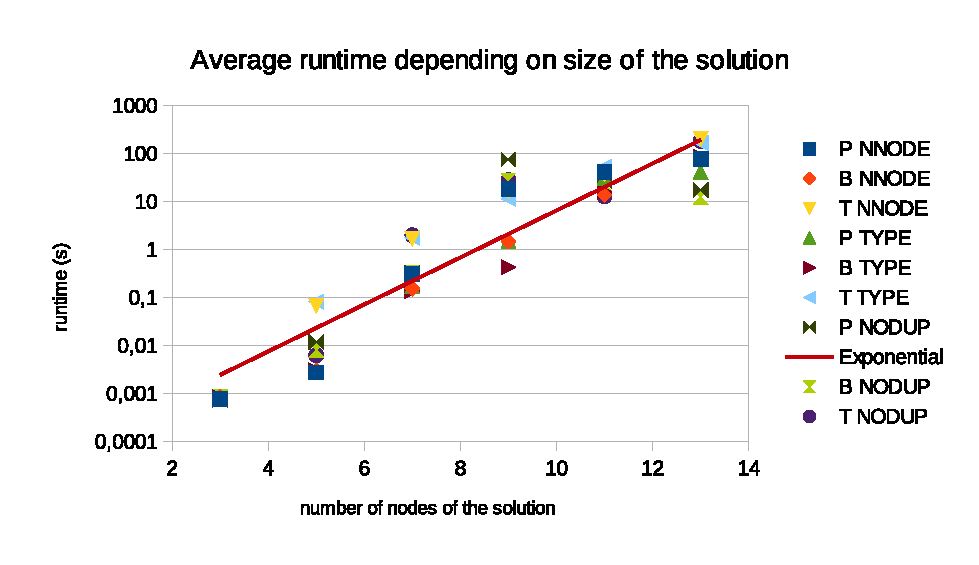
\includegraphics[width=0.95\textwidth]{time_vs_nof_nodes.eps}
    \caption{Average running time of the variants of the synthesis procedure depending on the number of nodes of the solution.}
    \label{fig:runtime_vs_nof_nodes}
\end{figure}
Figure~\ref{fig:runtime_vs_nof_nodes} shows that the average running time for all nine variants of the synthesis procedure depends exponentially on the number of nodes. This goes along with the intuition that a bigger program is more difficult to synthesise.
For example, if we have $n$ possibilities to generate a program consisting of one node, that is \lstinline!?x! where we have $n$ possibilities to instantiate the hole \lstinline!?x!, then we will have $n^2$ possibilities to generate a program with three nodes, that is \lstinline!?$x_1$ ?$x_2$! where we have $n$ possibilities to instantiate the hole.


\TODO{Delete this question or do something with it. We cannot answer it, we do not have enough data.}
More surprisingly, the individual results show that there must be some other factor influencing the runtime. Take, for example, \lstinline?enumFromTo?, \lstinline?stutter? and \lstinline?nth?. All three of them have a solution with exactly $13$ nodes, but their runtimes differ at least by an order of magnitude. What does make \lstinline?nth? generate in less than \SI{1}{s}, \lstinline?stutter? a hundred times slower and \lstinline?enumFromTo? to time out in most of the cases?

In our simple intuitive explanation of the exponential dependency of the synthesis time with the size of the solution we completely ignored the contribution of types to search space pruning.


\subsection{Type of the solution}
polymorphic easier to synthesise because less functions apply. nth vs stutter vs enumFromTo.
discuss together with type of components.

\TODO{why does enumFromTo take so much time even with enumTo as a component}
\TODO{we can actually synthesise enumFromTo without enumTo and we actually did in a very restricted context (only the library components present in the actual solution), but it takes a lot of time.}
\subsection{Number of components}
\subsection{Examples}
\subsection{Blacklist}
\subsection{Templates}
\subsection{Cost functions}
\subsection{Stack vs Queue expansion}

\section{Interesting unexpected solutions}
\TODO{explain the thing with the different solutions\\}
\TODO{discuss interesting solutions, isEven, member\\}
\TODO{polymorphic equality\\}
\section{Automatic black list}\label{Automatic black list}

\section{Comparison to related work}








----------------------------------------
What I want to see in this chapter:
\begin{itemize}
\item runtime highly dependent on the number of components used in the solution \TODO{if you have time, redo the graph relating number of components to runtime in latex}
\item difficult to find examples (small but enough)
Sensible to the choice of examples: for speed (enumTo prod enumTo prod...), examples must be small and there must be only a few of them. But then it is very likely, that another program is generated. It is very tricky to choose the right examples for enumFromTo and for member.
\item blacklist tradeoff: Show advantages of using black lists and explain why we do not see them in the data. (we do see them. Compare plain nof-nodes with blacklist nof-nodes. The benefit is comparable with the introduction of the nof-nodes-simple-types cost function. Which is reasonable, because they both fight against \lstinline?head nil?.)
\item Table of all components (no, this should go to implementation)
\item Table of synthesized programs with synthesis times for the different algorithms (aka giant-table-19 and giant-table-37)
\item Figure of the synthesis times of synthesized programs (nope)
\item Comparison to Feser, to Nadia, to Escher and to Myth (yes, we have their running times for some of the benchmarks. Say that you cannot really compare the numbers because they weren't run on the same machine).
\item Explain why automatic black list generation did not worked out as you wished
\begin{itemize}
\item only identity function (but you could also generate something else)
\item many "useless" programs already ruled out by other programs (but you could incrementally use the blacklist as a blacklist, you know?)
\item (maybe) show it?
\end{itemize}
\item Explain why templates perform so poorly (hm... because they don't do BFS, that is they have to explore every branch to the "end"?)
\item How number of components affects synthesis time
\begin{itemize}
\item In particular, not only the number but also the number of components of the same type. If you have more functions with the same type you will need much more time to find the program you are looking for (more possible successors).
\end{itemize} 
\item Talk about the constants in the cost functions and how they affect the search space.
How cost functions influence the search space (\lstinline!(head (^26 -> ^27 -> Int) (nil (^26 -> ^27 -> Int))) ?2 ?3! has too complicated types appearing in the term, so it will have a higher cost in some of the cost functions. \lstinline!foldnat foldnat foldnat mul (mul 3 3) 3! takes a lot of time to evaluate, it will have a higher cost in no-same-component).
\begin{itemize}
\item Idea behind nof-nodes: smaller programs generalize better to the examples
\item Idea behind nof-nodes-simple-types: programs with smaller types are less "useless" (example with \lstinline?head nil?). Favor the use of input variables. But now a lot of "simple" but difficult to evaluate programs are synthesised, like the \lstinline?enumTo prod enumTo prod?.
\item Idea behind no-same-component: there are components that are usually used only once in a program, like \lstinline?foldr?, \lstinline?foldNat?. Another thing is that we penalize also complicated types of the form \lstinline?List (List (^5 -> List ^4))? that had no additional cost in nof-nodes-simple-types. But now types overweight the number of nodes and simple programs like \lstinline?foldr add zero _0? weight more than programs like \lstinline?add mul sub prod enumTo...?.
\item Idea behind no-same-component-bigger-constants: make all constants bigger so that we can differentiate more between the constants and so that nodes count more than types.
\item Idea behind no-same-component-even-bigger-constants: see above. (well, then you failed. your constants for types are pretty much as big as those for terms...). Why it's bad? See above.
\end{itemize}
\item Stack versus queue expanding $\rightarrow$ mention it in the definitions (argument why stack is better. Intuitively it makes sense to construct a program from top-down or bottom-up, but it does not make any sense to put in some components in the middle. \lstinline!?1 ?2! gets transformed to \lstinline!(?3 ?4) ?2! and then we get programs like \lstinline!(?3 ?4) sum! and \lstinline!(?3 ?4) foldr! for all possible components. The leftmost strategy makes much more sense, because then we put constraint on the type of the next hole to be expanded.
\end{itemize}

\section{Set up}
  \note{Describe the machine and the testing set up, which components were used, what information did you give to the synthesizer, how many examples were given. What else?}
All experiments were run on an Intel quad core 3.2~GHz with 16~GB RAM. Since the code is sequential, the performance could not benefit from the number of cores.

We refer to Table~\ref{giant_table_19} and Table~\ref{giant_table_37} for the experimental results. All performance numbers are averages from 1 to 3 different executions all sharing the same specification. The goal type and the given examples do not change between different executions. In Table~\ref{giant_table_37} all benchmarks share the same set of components.

\section{Specification size}

\section{Solution size}
  
\section{Cost functions}
  \note{Compare the different cost functions with each other, explain why are they good for some programs and bad for other. Table.}

\section{Black lists}

In the presence of "useless" functions with a high branching factor like \lstinline?flip?, \lstinline?const? or \lstinline?uncurry? black list pruning is a must. But it can also be useful in other cases as well. The important thing is to find a reasonable trade off between the length of the black list (don't forget that every subterm of every open program is matched against every item of the black list) and the degree of pruning. A longer black list prunes more of the search space, but the synthesis procedure also takes longer.

  \subsection{Benefits of black lists}
  \note{Table of your super manual black list. Figure that for each cost function compares time with and without black list. Trivial words about pruning search space and useless branches.}
  \subsection{Shortcomes of automatically generated black lists}
  \note{Maybe really bring the automatically generated table. Point at the repetitions. Say that automatically generated I/O-examples are bad and we need a lot of them. Say that you tried only identity pruning, but one could also try to generate, say, the empty list or whatever.}

\section{Templates}
  \note{Short section explaining that the templates you generate are not the templates you expect and why}
I found one example, where templates help! For \lstinline?dropmax? I had a run out of memory exception with plain enumeration and I could synthesise it in 7 seconds with templates!
(Ok, I modified templates to put in only really higher-order components and close every hole, no matter the type).

It is very important to choose the examples well, because many generated programs are bad and will take forever to evaluate. And as we evaluate each closed program on the examples... We should really try to keep them small and simple.
For example, I had a problem when I tried to generate \lstinline?dropmax? using the example \lstinline?[1,4,3]?, because one of the generated programs was \lstinline?enumTo (prod (enumTo (prod _0)))?. It tried to construct a list with 479001600 elements and ran out of memory.
At the same time, they should give enough information, otherwise a simpler program will be generated that, although it satisfies all given I/O-examples, it not what the user had in mind when writing the specification.

%%% Local Variables:
%%% mode: latex
%%% TeX-master: "thesis"
%%% End:
